\section*{Assignment 01: Platform Concept and Value Proposition}
\addcontentsline{toc}{section}{Assignment 01: Platform Concept and Value Proposition}

The platform we built, \textbf{SkillSync}, connects students chasing real projects with small organisations that need help but lack consultant budgets. SkillSync is a digital infrastructure that facilitates repeated exchanges between distinct user groups \citep{Choudary2016}. Our core promise is a scoped collaboration that gives students portfolio wins while NGOs unlock motivated talent for a few intense weeks.

The concept only clicked after several iterations. Early notes just said ``students helping real-world actors,'' which classmates rightly called a slogan. Guided by \citet{Choudary2016} and \citet{Srnicek2017} we tightened the idea into a project-based platform between internships and gig work: flexible enough to dodge HR red tape yet structured enough to deliver measurable outcomes.

SkillSync therefore behaves as a two-sided orchestrator. Students bring skills and energy; NGOs and civic teams bring real problems. We focus on trustworthy matchmaking so cross-side network effects can blossom. Institutional email verification, lightweight vetting, and a templated scoping wizard keep expectations aligned before anyone spends serious time, exactly the launch hygiene emphasised in Lecture~2 on platform network effects \citep{Lecture02}.

Data is the quiet engine. Every project generates feedback, endorsements, and behavioural signals. In the short run we refine matching; in the longer run we craft portable skill passports, giving us an edge in the credentialing space \citet{Zuboff2019} critiques. The value proposition sits inside those loops as much as in the pitch deck.

Figure~\ref{fig:student-view} keeps the promise tangible. The refreshed student dashboard highlights curated projects while pinning progress nudges and mentor notes on the right. Project cards emphasise stipend range, time commitment, and deliverables because uncertainty kills motivation, and the ``mentor check-in'' strip pulls past data so guidance stays personal.

\begin{figure}[H]
  \centering
  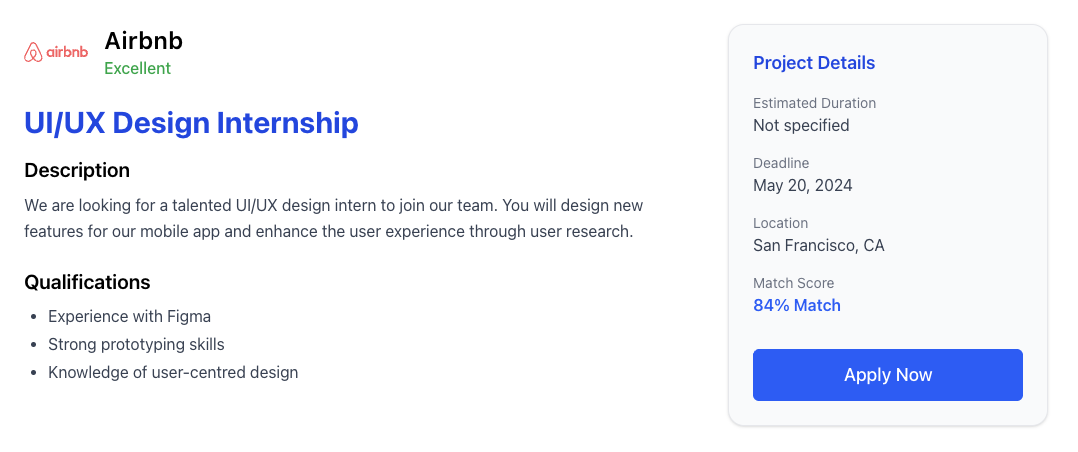
\includegraphics[width=0.85\linewidth]{Student-Project-View.png}
  \caption{Student project workspace with progress nudges.}
  \label{fig:student-view}
\end{figure}

On the supply side we created a mirrored experience for NGOs. The creation wizard walks through a scoping checklist in plain language: desired outcome, must-have skills, support on offer. We tested the template with our two anchor NGOs until they could complete it in under eight minutes. The figure in Assignment~3 shows that workflow in action. The value proposition is therefore more than a slogan about ``students meet projects''; it is a set of micro-interactions that reduce uncertainty for both sides and make repeat usage more likely.

This expanded Assignment~1 shows how SkillSync translates course concepts into practice. We centre one core interaction, leverage network effects, keep marginal costs tiny, and treat fairness as a strategic asset. The platform is not a generic marketplace; it is a carefully orchestrated arena where early-career value emerges through trust-rich collaboration.
